\documentclass[]{article}
\usepackage{amsmath}
\usepackage{amssymb}
\usepackage{graphicx}
\usepackage{subfig}
\usepackage{epstopdf}
\usepackage{inputenc}
\usepackage[margin=0.5in]{geometry}
\usepackage{titling}
\newcommand{\subtitle}[1]{%
	\posttitle{%
		\par\end{center}
	\begin{center}\large#1\end{center}
	\vskip0.5em}%
}
\usepackage{hyperref}
\hypersetup{
	colorlinks=true,
	linkcolor=blue,
	filecolor=magenta,      
	urlcolor=cyan,
	pdftitle={Overleaf Example},
	pdfpagemode=FullScreen,
}

\urlstyle{same} 

% Title Page
\title{Predicting Wine Quality From Wine Chemistry}
\subtitle{Modeling Red and White Wine}

\author{Robert V. Moel}

\begin{document}
\maketitle
\newpage
\begin{abstract}
Wine is loved by people from around the world.  Being able to use wine chemistry to determine wine quality would speed selection and permit for a tasty repast.
\end{abstract}
\newpage
\section{Data Source, EDA, and Preprocessing}
The source of data used for this evaluation comes from \url{https://archive.ics.uci.edu/ml/machine-learning-databases/wine-quality/}  This data table consists of the following


\begin{table}[ht]
	\centering
	\begin{tabular}{|l | l|}
		\hline
		Name of Parameter & Value Type \\
		\hline
		Fixed acidity & Real\\
		Volatile acidity &  Real\\
		Citric Acid &  Real\\
		Residual sugar &  Real\\
		Chlorides &  Real\\
		Free sulfur dioxide &  Real\\
		Total sulfur dioxide &  Real\\
		Density &  Real\\
		pH &  Real\\
		Sulphates &  Real\\
		Alcohol &  Real\\
		Quality (score between 0 and 10) &  Integer \\
		\hline	
	\end{tabular}		
\end{table}
The data is presented in two tables: one for red (1599 rows) and one for white (4898 rows) with 12 different attributes - 11 explanatory attributes and 1 predictive attribute called "quality."  Each wine's quality is ranked from 1 through 10 with 10 representing a wine with the highest quality based on a human taster.  For the analysis, an additional column, color, was added to each table where, 1 means a red wine and 0 means a white wine.  The tables were then joined together to create a single table to analyze.  Both tables were very complete and no row contained missing data.

Descriptive statistics where run on the data with the following results:
\begin{table}[ht]
	\centering
	\begin{tabular}{|l | r| r | r | r | r | r | r | r |}
		\hline
                    &   Count  &      Mean &       Std &     Min  &     25\% &          & 75\%       & Max        \\
\hline
Fixed acidity       &  6497.0  &  7.215307 &  1.296434 & 3.80000  & 6.40000  & 7.00000  &   7.70000  & 15.90000   \\
Volatile acidity    &  6497.0  &  0.339666 &  0.164636 & 0.08000  & 0.23000  & 0.29000  &   0.40000  &  1.58000   \\
Citric acid         &  6497.0  &  0.318633 &  0.145318 & 0.00000  & 0.25000  & 0.31000  &   0.39000  &  1.66000   \\
Residual sugar      &  6497.0  &  5.443235 &  4.757804 & 0.60000  & 1.80000  & 3.00000  &   8.10000  & 65.80000   \\
Chlorides           &  6497.0  &  0.056034 &  0.035034 & 0.00900  & 0.03800  & 0.04700  &   0.06500  &  0.61100   \\
Free sulfur dioxide &  6497.0  & 30.525319 & 17.749400 & 1.00000  &17.00000  & 29.00000 &   41.00000 & 289.00000  \\
Total sulfur dioxide&  6497.0  &115.744574 & 56.521855 & 6.00000  &77.00000  & 118.00000&   156.00000&  440.00000 \\ 
Density             &  6497.0  &  0.994697 &  0.002999 & 0.98711  & 0.99234  & 0.99489  &   0.99699  &  1.03898   \\
pH                  &  6497.0  &  3.218501 &  0.160787 & 2.72000  & 3.11000  & 3.21000  &   3.32000  &  4.01000   \\
Sulfates           &  6497.0  &  0.531268 &  0.148806 & 0.22000  & 0.43000  & 0.51000  &   0.60000  &  2.00000   \\
Alcohol             &  6497.0  & 10.491801 &  1.192712 & 8.00000  & 9.50000  & 10.30000 &   11.30000 &  14.90000  \\
Quality             &  6497.0  &  5.818378 &  0.873255 & 3.00000  & 5.00000  & 6.00000  &   6.00000  &  9.00000   \\
Wine{\_}color       &  6497.0  &  0.753886 &  0.430779 & 0.00000  & 1.000    & 1.00000  &   1.00000  &  1.0000000 \\  
		\hline	
\end{tabular}		
\end{table}

 \begin{figure}
 	\begin{tabular}{cccc}
 		\subfloat[caption]{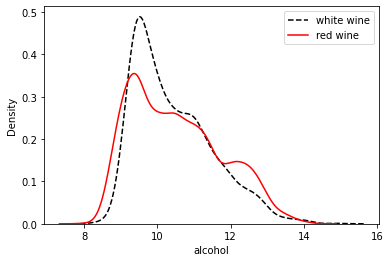
\includegraphics[width = 1.5in]{../image/densAlch.png}} &
 		\subfloat[caption]{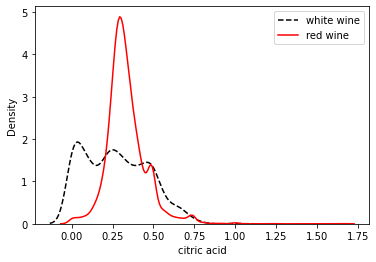
\includegraphics[width = 1.5in]{../image/densCitricAcid.png}} &
 		\subfloat[caption]{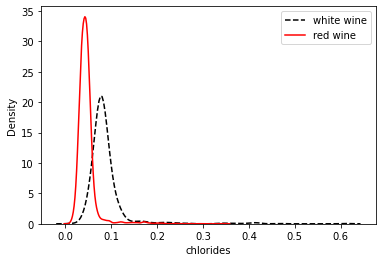
\includegraphics[width = 1.5in]{../image/densClorides.png}} &
 		\subfloat[caption]{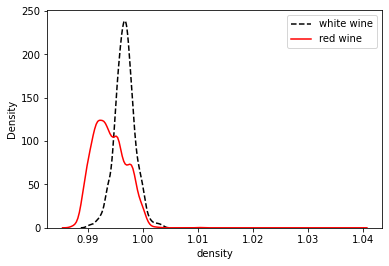
\includegraphics[width = 1.5in]{../image/densDensity.png}}\\
 		\subfloat[caption]{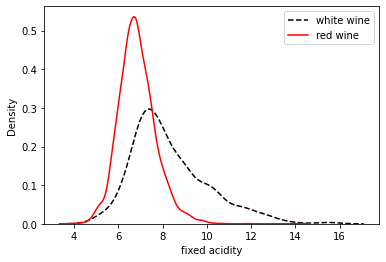
\includegraphics[width = 1.5in]{../image/densFixedAcid.png}} &
 		\subfloat[caption]{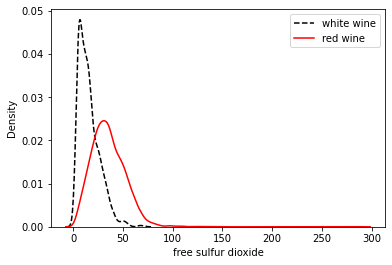
\includegraphics[width = 1.5in]{../image/densFreeSulf.png}} &
 		\subfloat[caption]{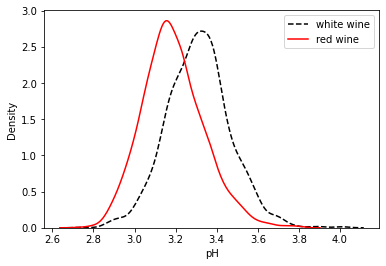
\includegraphics[width = 1.5in]{../image/denspH.png}} &
 		\subfloat[caption]{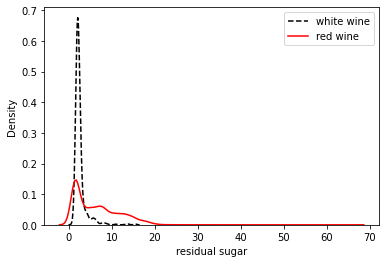
\includegraphics[width = 1.5in]{../image/densResidSugar.png}}\\
 		\subfloat[caption]{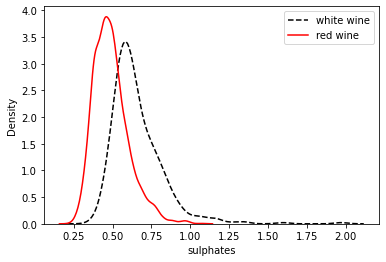
\includegraphics[width = 1.5in]{../image/densSulphates.png}} &
 		\subfloat[caption]{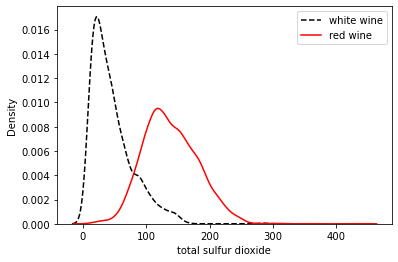
\includegraphics[width = 1.5in]{../image/densTotSulf.png}} &
 		\subfloat[caption]{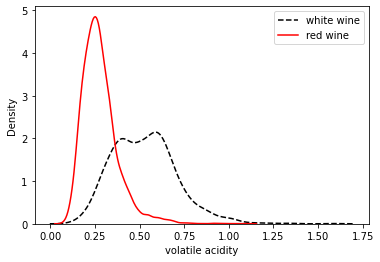
\includegraphics[width = 1.5in]{../image/densVolAcid.png}}

 	\end{tabular}
 	\caption{Density Plots of Red and White Wines}
 \end{figure}
  
We can see from these density plots that the data are not particularly normal. Let's look at two versions of the correlation heat map.
 \begin{figure}
	\begin{tabular}{c}
		\subfloat[Heat Map]{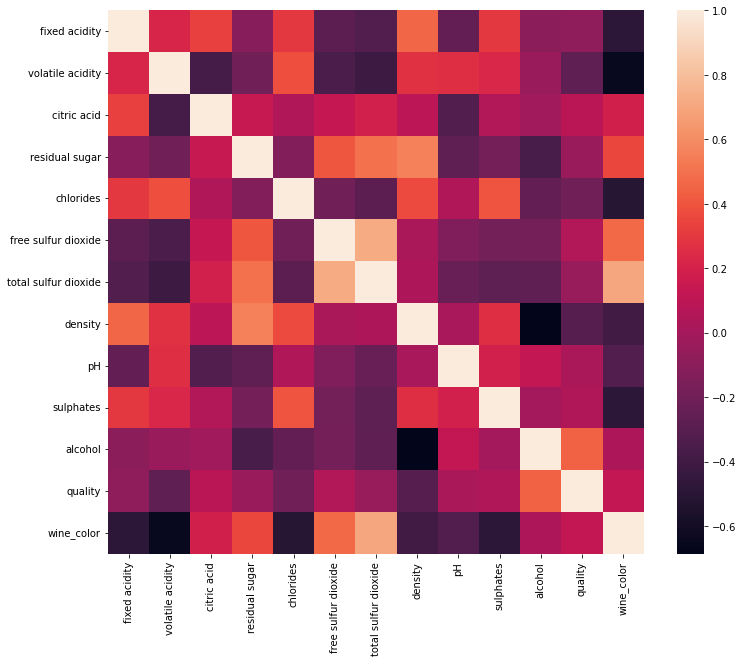
\includegraphics[width = 5in]{../image/heatmapall.png}} \\
		\subfloat[Correlation]{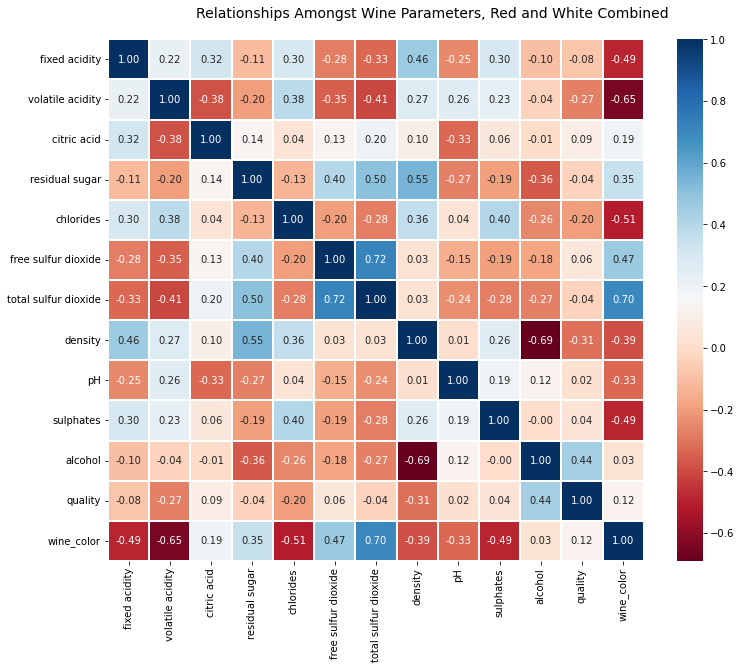
\includegraphics[width = 5in]{../image/corrheatmap.png}}
	\end{tabular}
	\caption{Heat Maps}
\end{figure}  
  
Some explanatory variables are not independent.  As expected, measures of acidity are related

Let's look at a pair-plots diagram to get a better look at some of these relationships:

    \begin{figure}
    	\begin{tabular}{c}
    		\subfloat[caption]{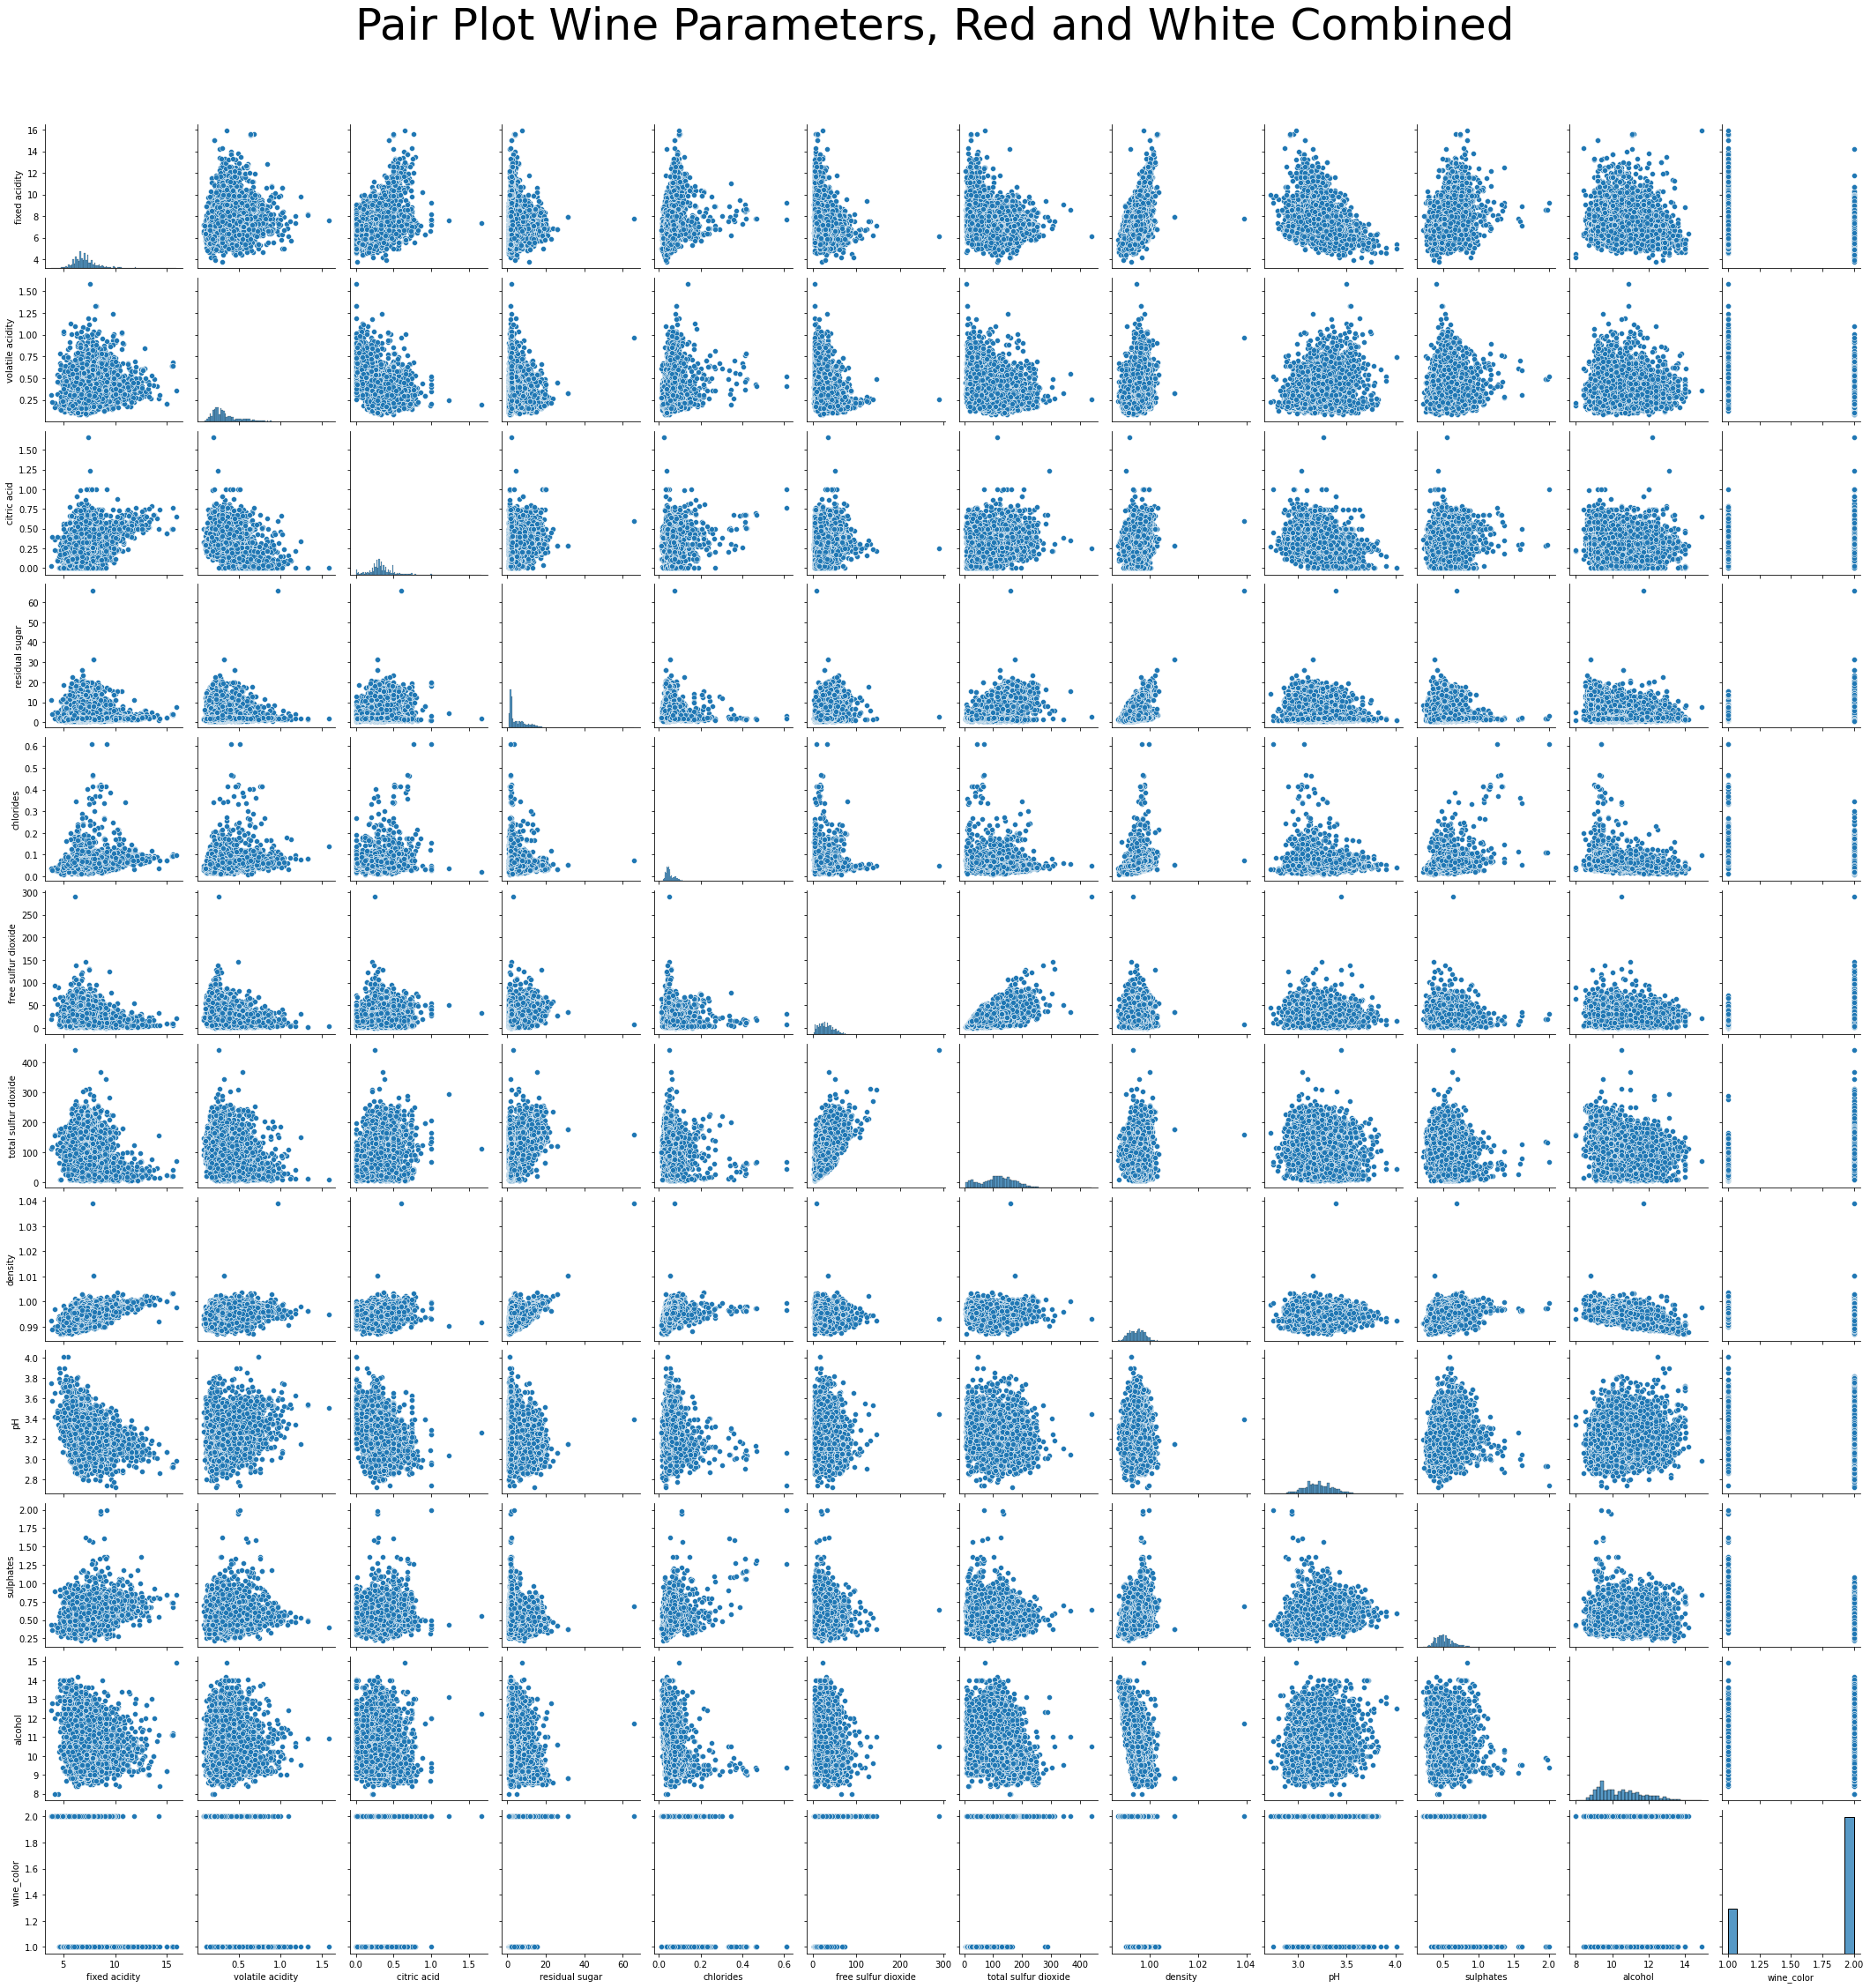
\includegraphics[width = 7in]{../image/pairplot.png}} 
    	\end{tabular}
    	\caption{Pair Plots}
    \end{figure}  
  
The data are now ready to be used in modeling.

\section{Modeling Approaches}
Several modeling approaches will be tried to determine if chemistry can be used to find wine quality for both read and white whites.  The methods to be considered will be ordered logistic regression with ordered probit kernel, logistic regression with logit kernel, ordered logit kernel, a plain random forest regressor, and a tuned random forest regressor.  First, the data will be scaled, and a training and test sample will be drawn.  This will be used to find appropriate models. 
  
\subsection{Choosing Test and Training}  
To ensure we get a representative sample of each wine score and each wine color, the training and test data are created using a stratification variable created from wine{\_}color and from each of the quality scores.  Twenty-percent of the data were set aside as test. The dummy stratifying variable was then removed.  The training data were then scaled using StandardScaler and this was applied to the test data.  
  
\subsection{Order Logistic Model}
The first ordered logistic model included all explanatory variables.  The model output is included below:

    \begin{figure}
	\begin{tabular}{c}
		\subfloat[caption]{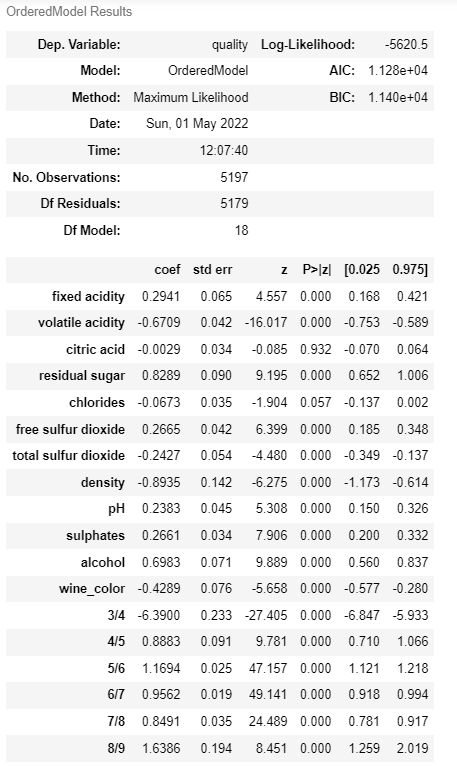
\includegraphics[width = 5in]{../image/LogitModel1.png}} 
	\end{tabular}
	\caption{First Logit Model}
\end{figure}
    
From this first run, we can see that citric acid and chlorides are not significant and can be dropped.

    \begin{figure}
	\begin{tabular}{c}
		\subfloat[caption]{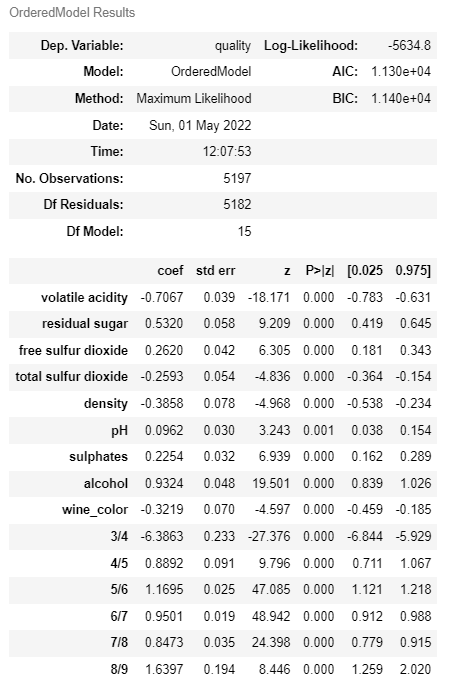
\includegraphics[width = 5in]{../image/LogitModel2.png}} 
	\end{tabular}
	\caption{Second Logit Model}
\end{figure}
This model appears to have all variables as significant.  Let's use this model against the test data and see how well it does in predicting quality.  An output of the multi-label confusion matrix is as follows: 
\begin{table}[h]
\centering
	\begin{tabular}{|l | r| r | r | r | r |}
		\hline
Label & Precision & Recall & Specificity & Accuracy & F1 \\
\hline		
3 & 1.0000 & 0.9915 & 0.0000 & 0.9915 & 0.9957 \\
4 & 1.0000 & 0.9700 & 1.0000 & 0.9700 & 0.9848 \\
5 & 0.8126 & 0.8045 & 0.5901 & 0.7377 & 0.8085 \\
6 & 0.4743 & 0.6772 & 0.5233 & 0.5831 & 0.5579 \\
7 & 0.9474 & 0.8544 & 0.4184 & 0.8215 & 0.8985 \\
8 & 0.9992 & 0.9723 & 0.0000 & 0.9715 & 0.9856 \\
9 & 1.0000 & 0.9969 & 0.0000 & 0.9969 & 0.9984 \\
\hline
\end{tabular}		
\end{table}
From this table we can see that labels at either end of the quality spectrum do well but labels in the center have difficulty determining average wines.  Overall, on the test y variables the model correctly predicts the quality 53.6\% of the time.

\subsection{Ordered Probit Model}
Let's use a probit kernel and see if this performs better using the same subset of variables as the second logit model.

    \begin{figure}
	\begin{tabular}{c}
		\subfloat[caption]{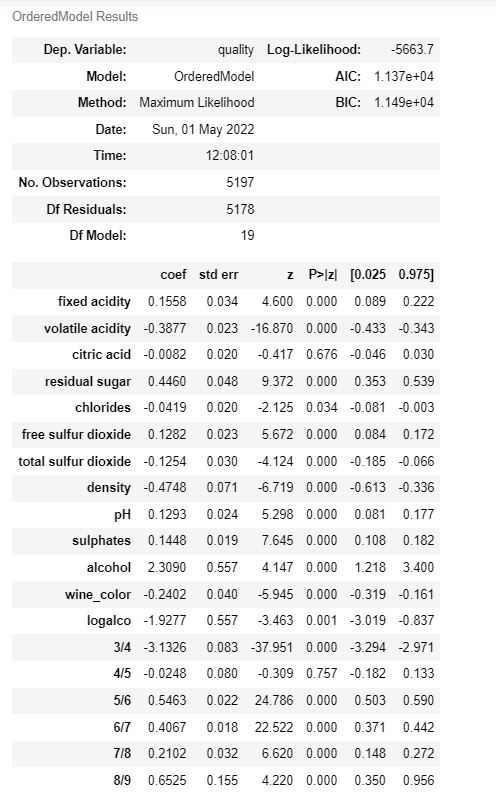
\includegraphics[width = 5in]{../image/ProbitModel1.png}} 
	\end{tabular}
	\caption{First Probit Model}
\end{figure}    

From this we can see the model is valid and all explanatory variables are significant.  Let's look at the results of the multi-label confusion matrix and the overall accuracy:
\begin{table}[h]
	\centering
	\begin{tabular}{|l | r| r | r | r | r |}
		\hline
		Label & Precision & Recall & Specificity & Accuracy & F1 \\
		\hline		
3 & 1.0000 & 0.9915 & 0.0000 & 0.9915 & 0.9957 \\ 
4 & 1.0000 & 0.9692 & 0.0000 & 0.9692 & 0.9844 \\ 
5 & 0.8036 & 0.8000 & 0.5756 & 0.7292 & 0.8018 \\ 
6 & 0.4674 & 0.6634 & 0.5152 & 0.5731 & 0.5484 \\ 
7 & 0.9456 & 0.8527 & 0.3980 & 0.8185 & 0.8968 \\ 
8 & 1.0000 & 0.9723 & 0.0000 & 0.9723 & 0.9860 \\ 
9 & 1.0000 & 0.9969 & 0.0000 & 0.9969 & 0.9984 \\ 
\hline
\end{tabular}		
\end{table}
 
 The overall ability to correctly predict quality for this model was 52.5\% not much better.  Again, we see weakness in its ability to predict in the middle quality score region.

\subsection{Random Forest Regressor}
Let's look at an untuned random forest regressor and we use the default values and max{\_}depth of 2.  Running this regressor and checking its ability to predict quality it does so about 51.6\% of the time which, isn't much better than a standard logistic regression.

\subsection{Tuned Random Forest}
In this next model we tune the following parameters: n{\_}estimators, max{\_}features, max{\_}depth, min{\_}samples{\_}split, and min{\_}samples{\_}leaf.  We set bootstrap to True. We used 5-fold cross-validation.


The best parameters are:
\begin{table}[h]
	\centering
	\begin{tabular}{|l | r|}
		\hline
		Hyper-parameter & Value\\
		\hline		
		Bootstrap & True \\ 
		Max Depth & 43 \\ 
		Max Features & Auto  \\ 
		Min Samples Leaf & 1 \\ 
		Min Samples Split & 2  \\ 
		N Estimators & 134  \\ 
		\hline
	\end{tabular}		
\end{table}

The overall accuracy of this model is 64.5\% or 10-percentage points higher than logistic regression

A visual of the tree is produced below:
    \begin{figure}[ht]
	\begin{tabular}{c}
		\subfloat{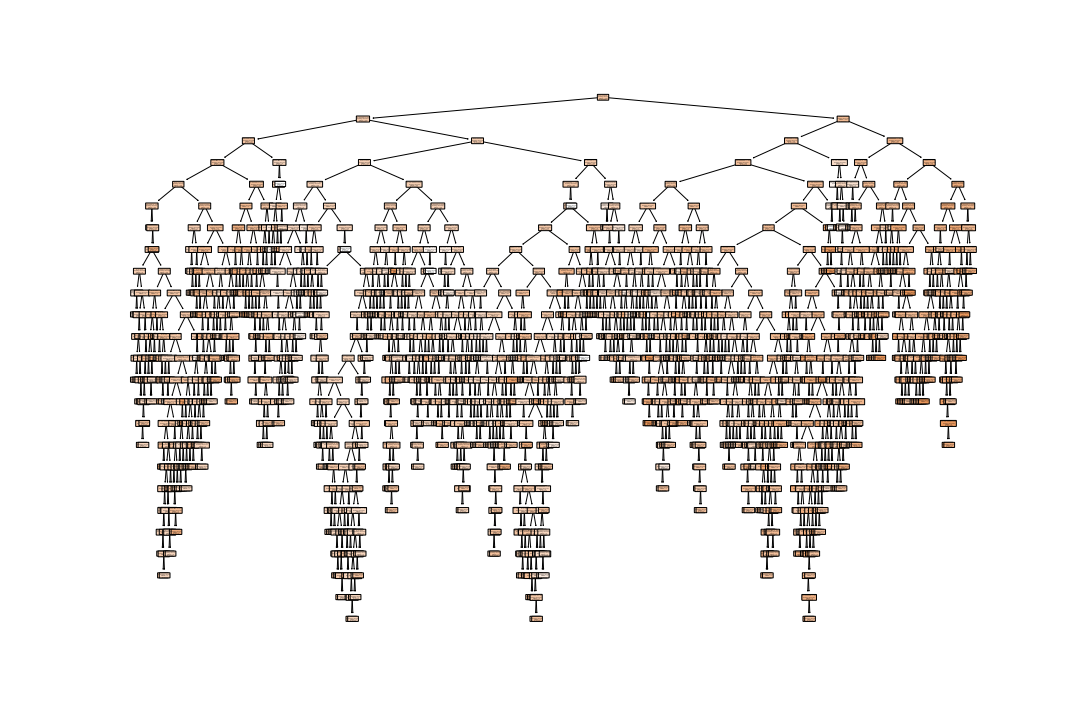
\includegraphics[width = 7in]{../image/regr_tree.png}} 
	\end{tabular}
	\caption{Tuned Tree Regressor Model}
\end{figure}

The confusion matrix produced the following results for each of the quality levels:
\begin{table}[h]
	\centering
	\begin{tabular}{|l | r| r | r | r | r |}
		\hline
		Label & Precision & Recall & Specificity & Accuracy & F1 \\
		\hline		
3 & 1.0000 & 0.9915 & 0.0000 & 0.9915 & 0.9957 \\ 
4 & 1.0000 & 0.9700 & 1.0000 & 0.9700 & 0.9848 \\ 
5 & 0.8488 & 0.8714 & 0.6934 & 0.8115 & 0.8600 \\ 
6 & 0.6630 & 0.7772 & 0.6453 & 0.7077 & 0.7156 \\ 
7 & 0.9327 & 0.8979 & 0.5805 & 0.8554 & 0.9150 \\ 
8 & 1.0000 & 0.9746 & 1.0000 & 0.9746 & 0.9871 \\ 
9 & 1.0000 & 0.9969 & 0.0000 & 0.9969 & 0.9984 \\
\hline
\end{tabular}		
\end{table}

What's clear here is that the random tree performs much better in the mid-range quality.  This improved the model's performance significantly.

\section{Further Research}
While 65\% is a great improvement over plain logistic regression models, better predictive power should be achievable with additional samples and not just Portuguese wine.  Because of the time it takes to tune this model, only a sample of hyper-parameters were tuned if more time and a more powerful CPU were available, more parameters could be tuned. The wines considered were Portuguese.  Additional wine nationalities should be included.  Additionally, only red or white were represented.  Ideally, rose should be added as a category.

\section{Top Three Recommendations on Using this Model}
First, this model can be used to identify great versus good wine brands from the thousands that are out there by just knowing the chemistry of the wine.  While this won't put great sommeliers out of work, it would help the average consumer find a great bottle of wine.  Second, this model can be used in the wine production and quality control process as a wine is produced and to help wines conform to chemistry that will make them taste better.  Finally, this model can be used to improve wines by adjusting their chemistry to wines that appear to taste better.  Because the model is tuned to both white and red wines, the specific tuning can be created   
    
\end{document}          
